\chapter{Global Planner}
\label{chap:global}

The task of the global planner is to assemble a specified target polyomino $\mathcal{T}$ given an initial configuration $g_\textit{init}$.
The configuration-space is explored by executing local plans developed by the local planner from \autoref{chap:local}.
That way, the part of the configuration-space we can actually explore is limited to configurations where a connection attempt between two cubes was made.
Compared to $SE(2)$ this part is manageable in size and only contains configurations which are relevant for self-assembly.

Determining how these configurations are explored affects the run time considerably.
Using rapidly-exploring random trees (RRTs) \cite{lavalle1998} yields good results in many cases, since the configuration-space gets evenly explored without the challenge of determining what decisions are promising for the end goal.
But it also explores many configurations which are not necessary for reaching the goal.
For us this approach is not reasonable. 
Because of the high fidelity simulation we are working with, the computation time for a local plan is huge, so planning the assembly of $\mathcal{T}$ with as few local plans as possible is the aim for our global planner.

We need to make well-thought-through connection decisions, that are valid for assembling $\mathcal{T}$, meaning some sort of building plan for a polyomino is needed.
Creating a building sequences by removing one tile at a time from the target was done by Becker et al.\ \cite{Becker2020}.
However, this does not consider sub-assemblies, so all cubes that are not to be connected have to stay separated at any time.

It is hard to prevent sub-assemblies with magnetic cubes following the rules of tilt, so our approach uses an enumeration of ways to cut a polyomino into two parts (\autoref{sec:twocutting}), which will be used for generating a so-called two-cut-sub-assembly graph (\autoref{sec:tcsa}).
This graph functions as a building instruction along side the exploration of the configuration-space.
\autoref{sec:connect_options} provides a closer look on the use of the graph for decision making and \autoref{sec:local_in_global} explains the usage of the local planner on a global scale. 
Finally \autoref{sec:global_algo} combines previous techniques to a global planning algorithm.
For the algorithm the number of cubes in the workspace is limited to the size of $\mathcal{T}$.
An explanation on why is this done and why the problem becomes more complex when working with extra cubes, is provided in \autoref{sec:more_cubes}.


\section{Two-Cutting Polyominoes}
\label{sec:twocutting}

\begin{figure}
	\centering
	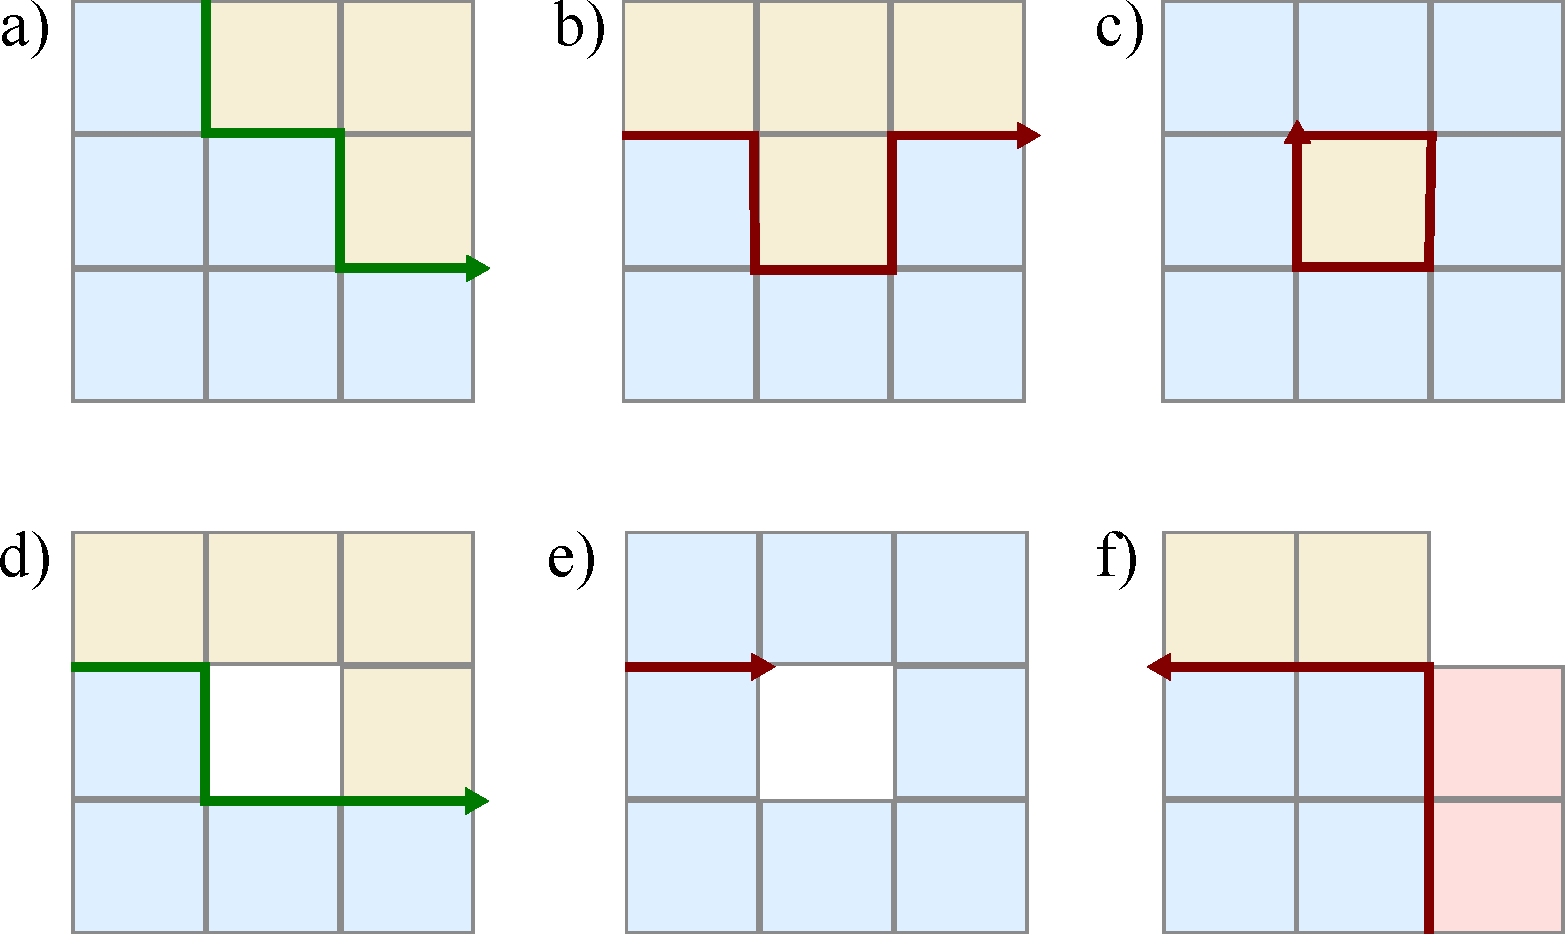
\includegraphics[width=0.6\textwidth]{figures/twocuts.pdf}
	\caption[Different cuts for polyomino shapes]{Examples for cutting polyomino shapes. a) to d) show three two-cuts for a $3\times3$ shape, of which only a) and d) are monotone and therefore valid. b) creates a cave and c) one a hole. e) and f) show cuts that do not split the polyomino into two pieces. e) does not break the polyomino at all and f) creates three sub-polyominoes.}
	\label{fig:twocuts}
\end{figure}

Schmidt et al.\ \cite{Schmidt2018} made use of straight-line two-cuts, to handle the construction of a polyomino with more than trivial sub-assemblies.

We define a two-cut as a continuous edge path through a polyomino that would divide the polyomino into two sub-polyominoes, if all connections with these edges are removed.
For later use in \autoref{sec:tcsa} we want to enumerate all two-cuts of a polyomino that are useful for planning.
We do not limit the cuts by only allowing straight paths like \cite{Schmidt2018}, instead we only consider monotone two-cuts.

\textit{Monotone} means that whenever the path goes into a direction it can never go into the opposite direction again.
\autoref{fig:twocuts} a) shows a monotone two-cut through a $3\times3$ polyomino shape.
The cut starts at the top of the shape and only moves down and right.
By removing all the connections on the path, the polyomino shape is split into two pieces.
Considering non-monotone two-cuts would create sub-assemblies with caves or holes, which could not be reassembled with our local planner.
For this reason they are omitted on a global scale in advance.
\autoref{fig:twocuts} b) shows a non-monotone two-cut creating a cave and \autoref{fig:twocuts} c) one creating a hole.

To calculate all two-cuts of a polyomino, we take all possible monotone paths from each connection as a starting point.
A path ends when it breaks out of the polyomino.
After the path ended the connection at its edges are removed from the polyomino and the path is added as a two-cut, if the polyomino got split into exactly two pieces.
\autoref{fig:twocuts} e) and f) show cuts that split the polyomino in less or more than two pieces.

% 32 possibilities for 3x3

\section{Two-Cut-Sub-Assembly Graph}
\label{sec:tcsa}

\begin{figure}
	\centering
	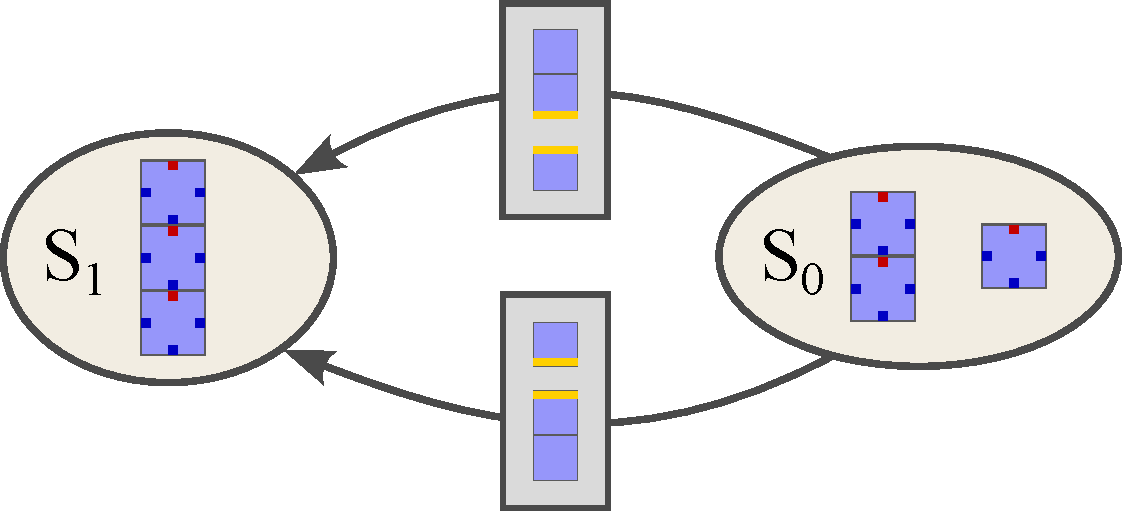
\includegraphics[width=0.45\textwidth]{figures/tcsa_multiedge.pdf}
	\caption[Two two-cut-sub-assembly nodes connected with multiple edges.]{Two two-cut-sub-assembly edges connecting the polyomino sets $S_0$ and $S_1$. The weights of the edges differ, since there are two ways to connect the $2\times1$ with the $1\times1$ to create a $3\times1$ polyomino. The connections are illustrated in rectangular boxes placed on the edges.}
	\label{fig:tcsa_multiedge}
\end{figure}

\begin{figure}
	\centering
	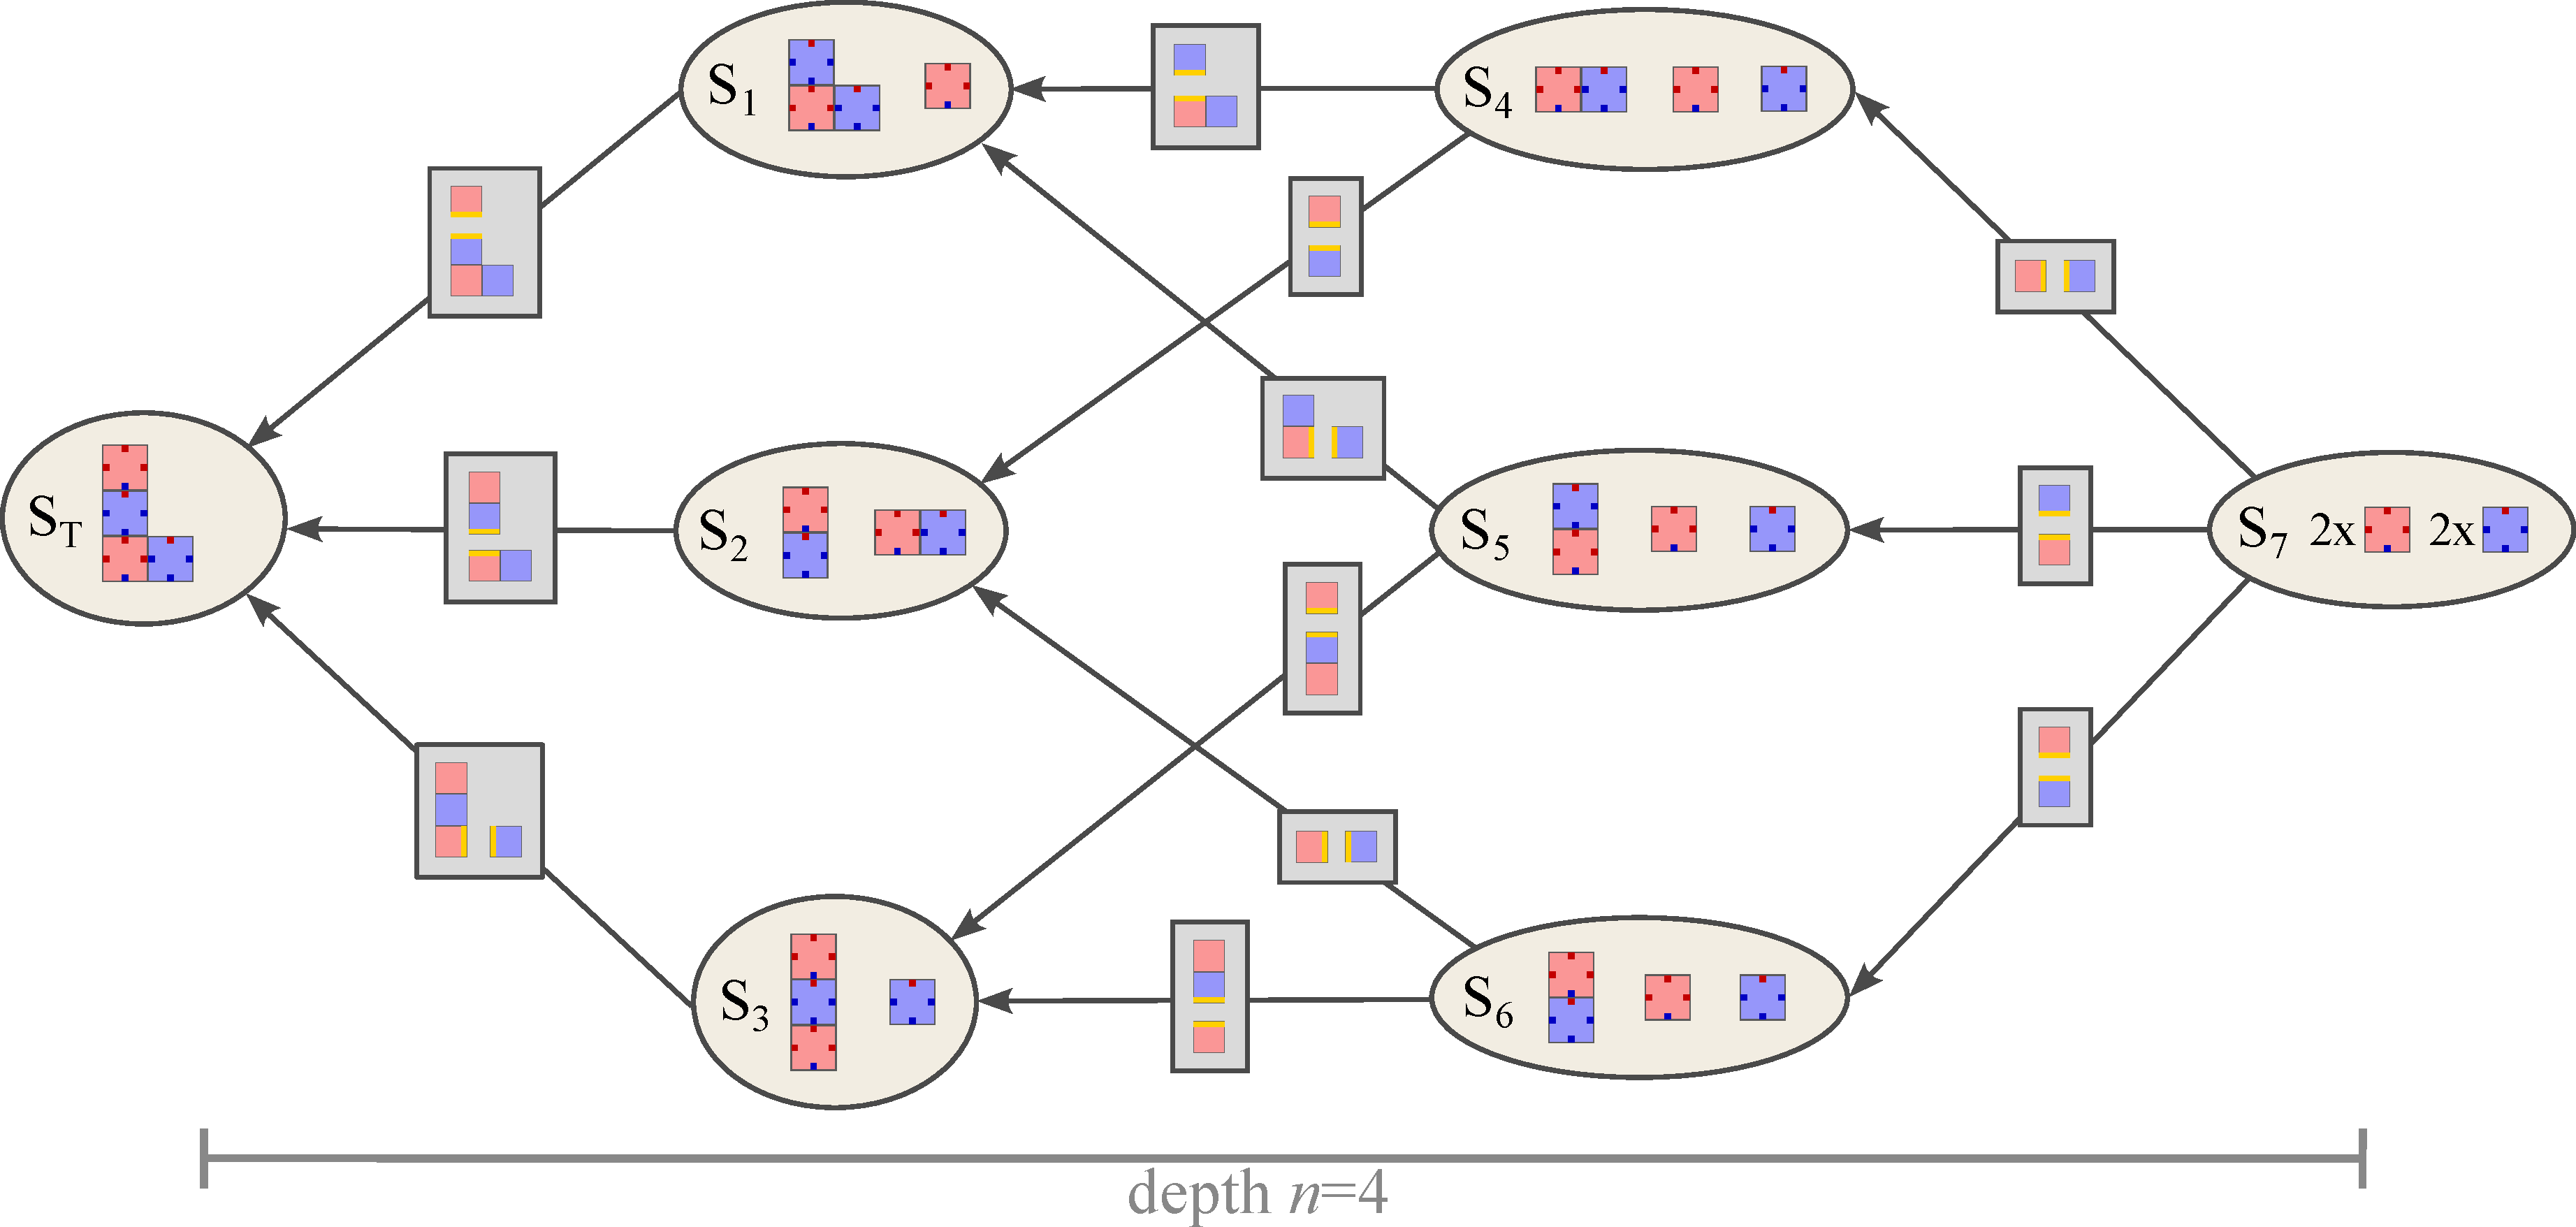
\includegraphics[width=1\textwidth]{figures/tcsa.pdf}
	\caption[Example for a two-cut-sub-assembly graph.]{Example of an two-cut-sub-assembly graph for a four-cube L-shape. The polyomino sets are illustrated as ellipses. If the polyominoes of a set are not numbered, there is only one occurrence of this polyomino. Otherwise the number of occurrences is placed left of the polyomino. The sets are numbered as if the graph was produced by \autoref{algo:build_tcsa} starting from $S_\mathcal{T}$. The weight of edges are illustrated as rectangular boxes containing the polyominoes that need to be connected at specific edges, marked in yellow.}
	\label{fig:tcsa}
\end{figure}
%TODO addglobal plan comic sequence and highlight path in graph

The two-cut-sub-assembly graph, short TCSA graph, functions as a building instruction for a specific target polyomino, we will call it $G_{\textit{TCSA}}(\mathcal{T}) = (V,E)$ represented by nodes $V$ and edges $E$.
The TCSA graph works with sets of polyominoes as nodes.
While a configuration $g$ holds information about orientation and position of physically distinct polyominoes, the corresponding polyomino set $S(g)$ only enumerates the polyomino types preset in $g$.
If $g$ contain multiple polyominoes of the same type, $S(g)$ still stores the amount of the polyomino type, but does not distinguish between the actual polyominoes.

Two nodes $S_0$ and $S_1$ of the TSCA graph are connected with an edge $\{S_0,t_c,S_1\}$, if $S_0$ can be transformed to $S_1$ by connecting two polyominoes contained in $S_0$.
The edge path specifying this connection is stored as the weight $t_c$.
$S_0$ and $S_1$ can be connected by multiple edges, if there are different connections that produce the same outcome.
The edges differ in their weights as shown in \autoref{fig:tcsa_multiedge}.
The direction of $\{S_0,t_c,S_1\}$ always goes from $S_0$ to $S_1$, but we can reverse the definition for an edge as following:

Two nodes $S_0$ and $S_1$ are connected, if one polyomino contained in $S_1$ can be two-cut by an edge path $t_c$, so that the resulting polyomino set equals $S_0$.
This already provides a perspective on the use of two-cuts and the way $G_{\textit{TCSA}}(\mathcal{T})$ is built starting with $\mathcal{T}$.
We will further explain the building process along with an example of a TCSA graph provided in \autoref{fig:tcsa}.


\paragraph{Building a TCSA Graph}

\begin{algorithm}
	\caption{$\text{\scshape Build-TCSA-Graph}$}
	\label{algo:build_tcsa}
	\begin{algorithmic}[1]
		\REQUIRE $\mathcal{T}$ \COMMENT{target polyomino}
		\ENSURE $G_{\textit{TCSA}}(\mathcal{T})$ \COMMENT{the graph is represented by nodes $V$ and edges $E$} 
		\STATE $V \gets \{\}$
		\STATE $E \gets \{\}$
		\STATE $i \gets 0$
		\STATE $V[i] \gets S_\mathcal{T}$ \COMMENT{start with set only containing $\mathcal{T}$}
		\WHILE[work through nodes in BFS manner]{$i < \text{\scshape Size}(V)$}
			\STATE $S_i \gets V[i]$
			\FOR[go through all polyomino types in $S_i$]{\textbf{each} $\mathcal{A} \in S_i$}
				\FOR[go through all monotone two-cuts]{\textbf{each} $t_c \in \text{\scshape Two-Cuts}(\mathcal{A})$}
					\STATE $(\mathcal{A}_1, \mathcal{A}_2) \gets \text{\scshape Cut-Polyomino}(\mathcal{A}, t_c)$
					\STATE $S_\textit{new} \gets \left( S_i \setminus \{\mathcal{A}\} \right) \cup \{\mathcal{A}_1, \mathcal{A}_2\}$ \COMMENT{new node after cutting}
					\IF{$S_\textit{new} \notin V$}
						\STATE $V \gets \text{\scshape Append}(V, S_\textit{new})$
					\ENDIF
					\STATE $E \gets \text{\scshape Append}(E, \{S_\textit{new}, t_c, S_i\})$
				\ENDFOR
			\ENDFOR
			\STATE $i \gets i+1$
		\ENDWHILE
		\RETURN $(V,E)$
	\end{algorithmic}
\end{algorithm}

\autoref{algo:build_tcsa} describes the process of building $G_{\textit{TCSA}}(\mathcal{T})$ for the target $\mathcal{T}$.
The algorithm works through each newly added node in $V$ in a breadth-first-search manner.
The first node added to $V$ is $S_\mathcal{T}$, which is a polyomino set only containing the target shape.

New nodes and edges are determined by two-cutting every polyomino type $\mathcal{A}$ in the current set $S_i$ by every possible monotone two-cut of $\mathcal{A}$.
This is done by enumerating the two-cuts with {\scshape Two-Cuts}, the way it was described in \autoref{sec:twocutting}, and cutting $\mathcal{A}$ at the two-cut with {\scshape Cut-Polyomino}.
The cutting results in the two sub-polyominoes $\mathcal{A}_1$ and $\mathcal{A}_2$.
$S_\textit{new}$ contains the same polyominoes as $S_i$ with the exception that one occurrence of $\mathcal{A}$ is removed and replaced by one occurrence of $\mathcal{A}_1$ and $\mathcal{A}_2$.
Each $S_\textit{new}$ is the result of cutting one polyomino of $S_i$ at a specific two-cut $t_c$.
If $S_\textit{new}$ is not already contained in $V$, we can add it to $V$, which also queues it for future iterations of the breadth-first-search.

No matter if $S_\textit{new}$ is contained in $V$ or not, an edge going from $S_\textit{new}$ to $S_i$ with $t_c$ as the weight is added to the graph edges $E$.
This allow multiple edges, as seen in \autoref{fig:tcsa_multiedge}, and multiple outgoing edges to different nodes, which can be observed in \autoref{fig:tcsa}, where different connections in $S_4$ lead to either $S_1$ or $S_2$.

Each two-cut applied to a polyomino set reduces its amount of polyominoes by one.
Let $n$ be the size of $\mathcal{T}$, then $n-1$ two-cuts applied to $S_\mathcal{T}$ will produce a polyomino set $S_\textit{trivial}$ containing only trivial polyominoes, as it is the case for $S_7$ in \autoref{fig:tcsa}.
All $S_i$ will inevitably end up in this situation and the algorithm will return $(V,E)$, since trivial polyominoes cannot be cut anymore.
This means that no matter which connections are chosen along the way, $n-1$ edges will always be needed to get from $S_\textit{trivial}$ to $S_\mathcal{T}$.
We describe this attribute, by giving the TCSA graph a depth of $n$.
The depth is also illustrated in \autoref{fig:tcsa} and the numbering of the nodes matches the order they were added by \autoref{algo:build_tcsa}.

\subsection{Complexity}

\begin{figure}
	\centering
	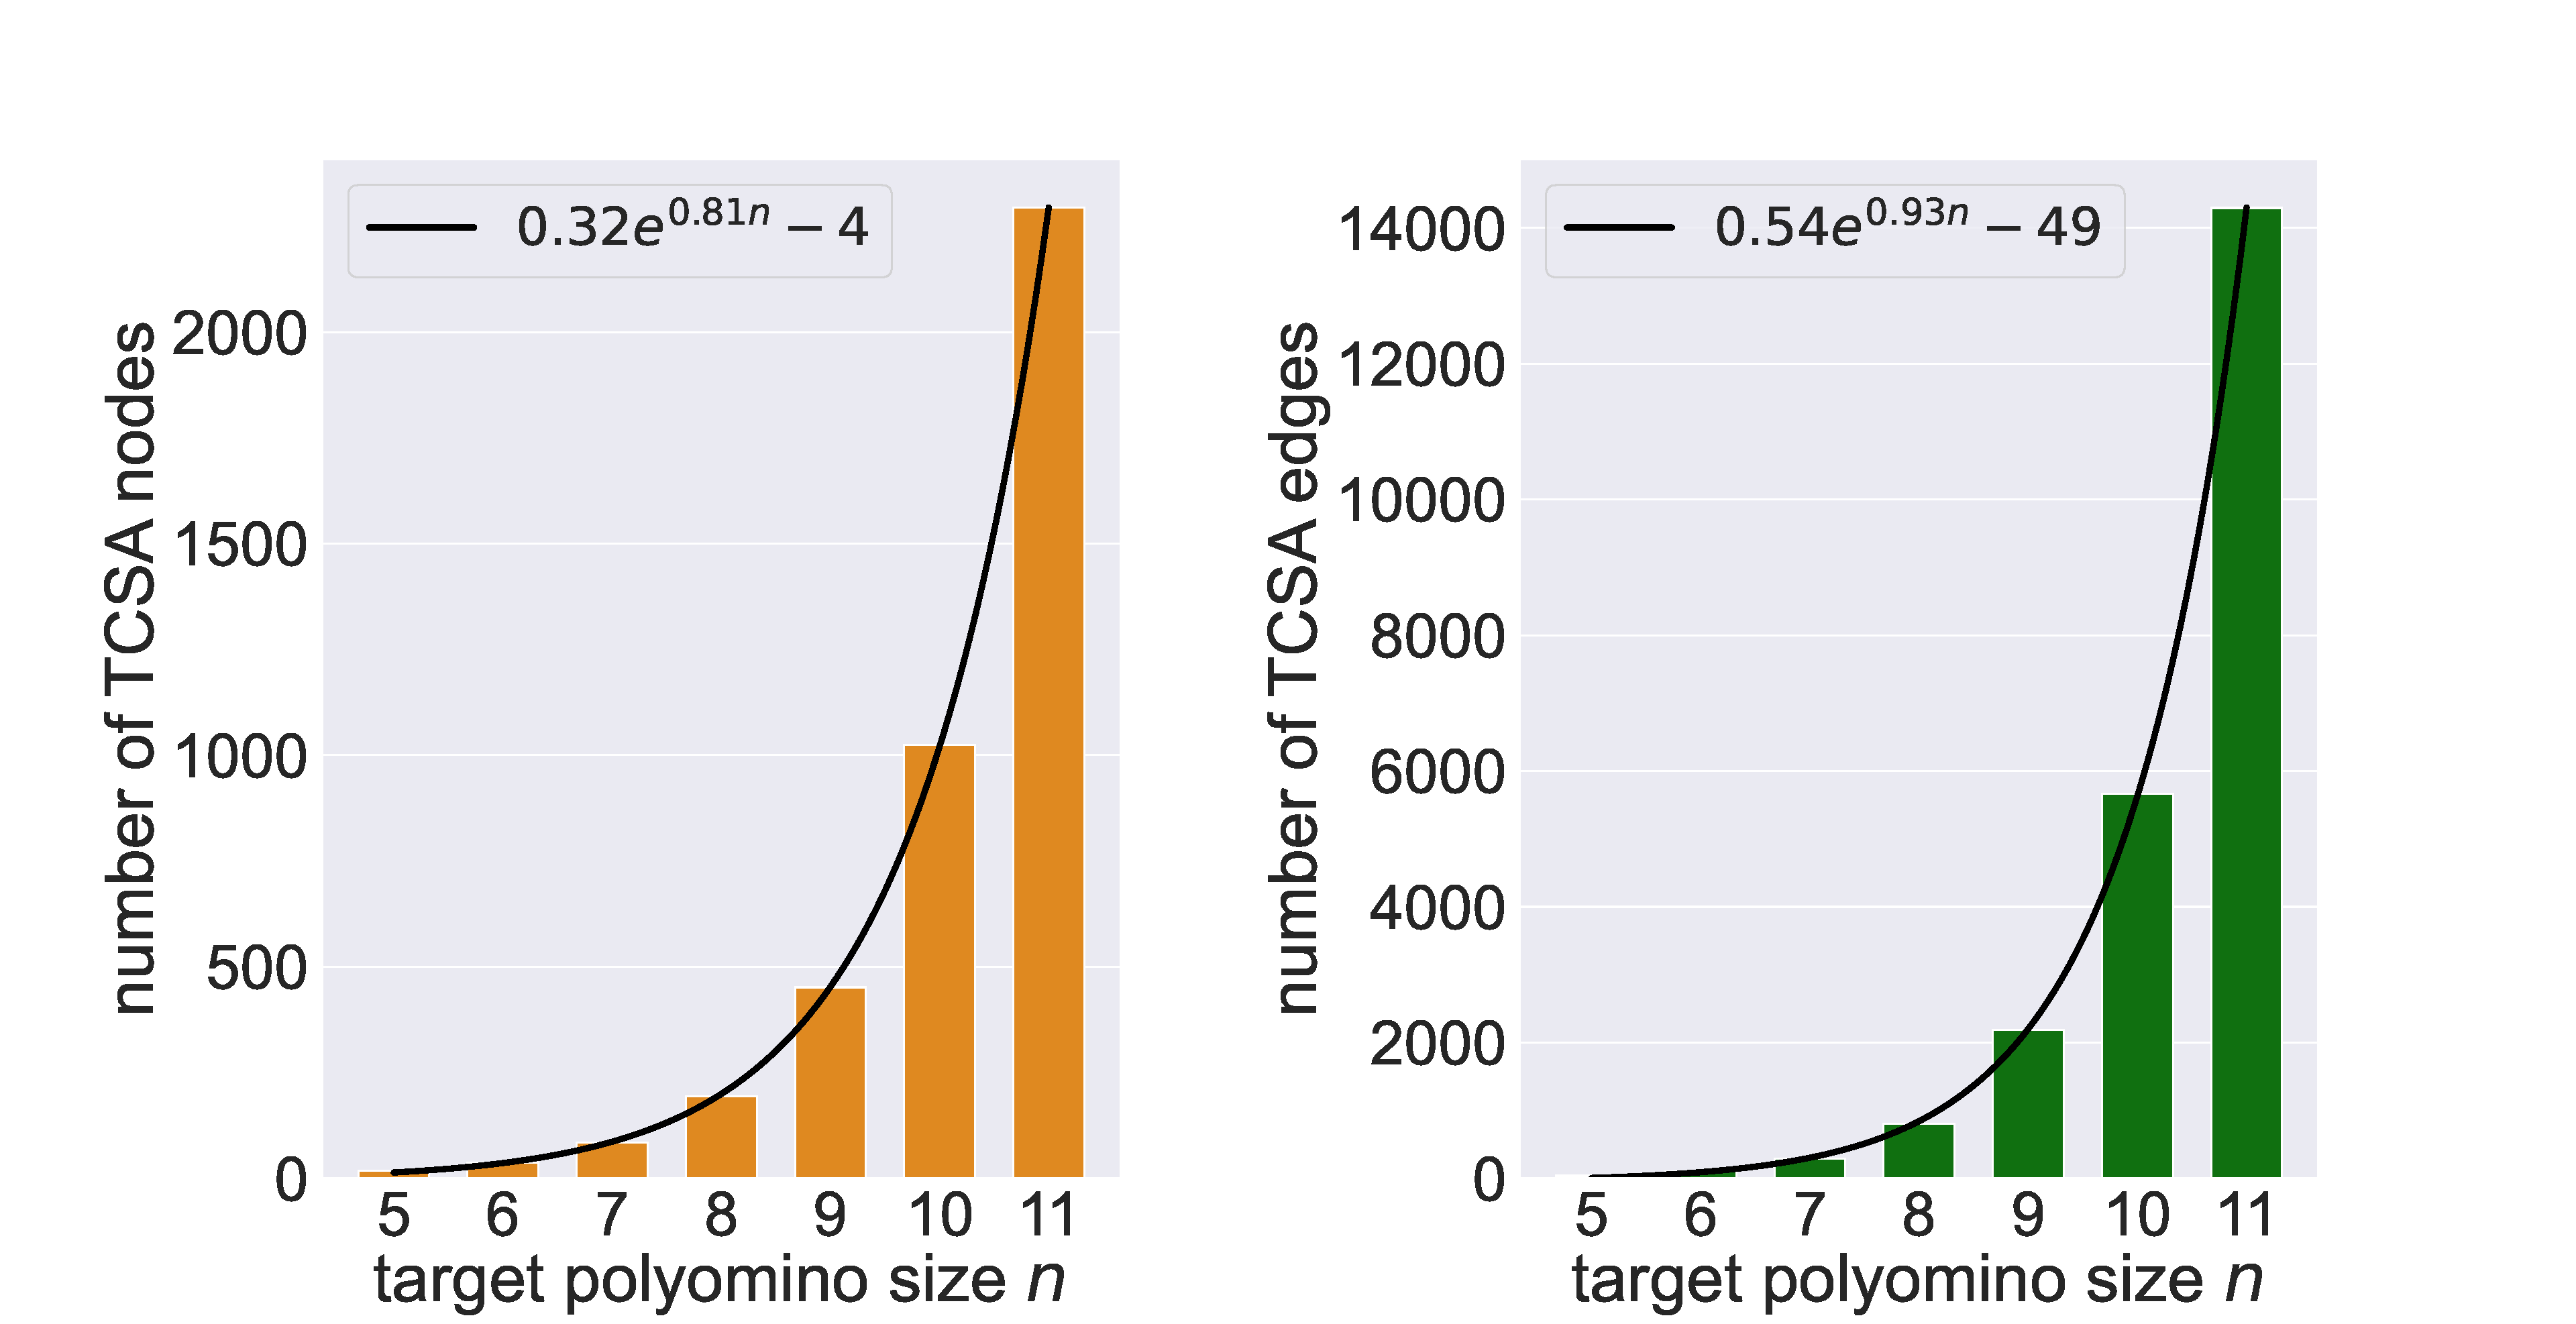
\includegraphics[width=0.8\textwidth]{figures/plots/tcsa_nodes_edges.pdf}
	\caption[Average two-cut-sub-assembly nodes and edges for target size $n$.]{Average number of nodes (left) and edges (right) of a TCSA graph for different target sizes $n$. For each $n$ $200$ samples of randomly generated polyominoes were taken. An exponential function is fitted over the averages of nodes and edges.}
	\label{fig:tcsa_plot}
\end{figure}

The Stirling numbers of second kind provide an upper bound for the number of nodes in a TCSA graph.
The Stirling numbers of second kind
\begin{equation}
\bracenom{n}{k} = \sum_{i=1}^{k} \frac{(-1)^{k-i} \, i^{n-1}}{(i-1)! \, (k-1)!}
\end{equation}
describe the possibilities of sorting a set with $n$ objects into $k$ partitions \cite{jelliss1991}.
In our case $n$ equals the target size $n$ and the number of partitions $k$ is the number of polyominoes, the $n$ cubes belong to.
Different layers of depth account for different $\bracenom{n}{k}$.
$S_\mathcal{T}$ is the only polyomino set with $k=1$, so $\bracenom{n}{1} = 1$.
$S_\textit{trival}$ is the only set containing $k=n$ polyominoes, so $\bracenom{n}{n} = 1$.
For the maximum number of nodes possible all layers of the TCSA graph have to be summed up
\begin{equation}
|V|_\textit{worst} = \sum_{k=1}^{n} \bracenom{n}{k} \, ,
\end{equation}
which is also referred to as the Bell number \cite{jelliss1991}.

In our case, the only way of sorting cubes into partitions is by monotonously two-cutting existing polyominoes, which drastically lowers the number of $|V|_\textit{worst}$.
In \autoref{fig:tcsa_plot} statistical data shows the average number of nodes and edges a TCSA graph consists of for varying target sizes $n$.
The growth of nodes and edges seems to be exponential, which is show with fitted functions in \autoref{fig:tcsa_plot}. 

Our implementation of $G_{\textit{TCSA}}(\mathcal{T})$ stores nodes in a hash-table.
Accessing nodes and connected edges, or checking if a polyomino set is contained in $G_{\textit{TCSA}}(\mathcal{T})$, can be done in  $\mathcal{O}(1)$.
The creation of $G_{\textit{TCSA}}(\mathcal{T})$ becomes more complex for increasing numbers of $n$, but it provides an easily accessible building instruction that drastically cuts the number of unnecessary local plans simulated.
Lowering simulation time makes a complex data-structure like the TCSA graph worth the extra effort.


\section{Connection Options}
\label{sec:connect_options}

\begin{figure}
	\centering
	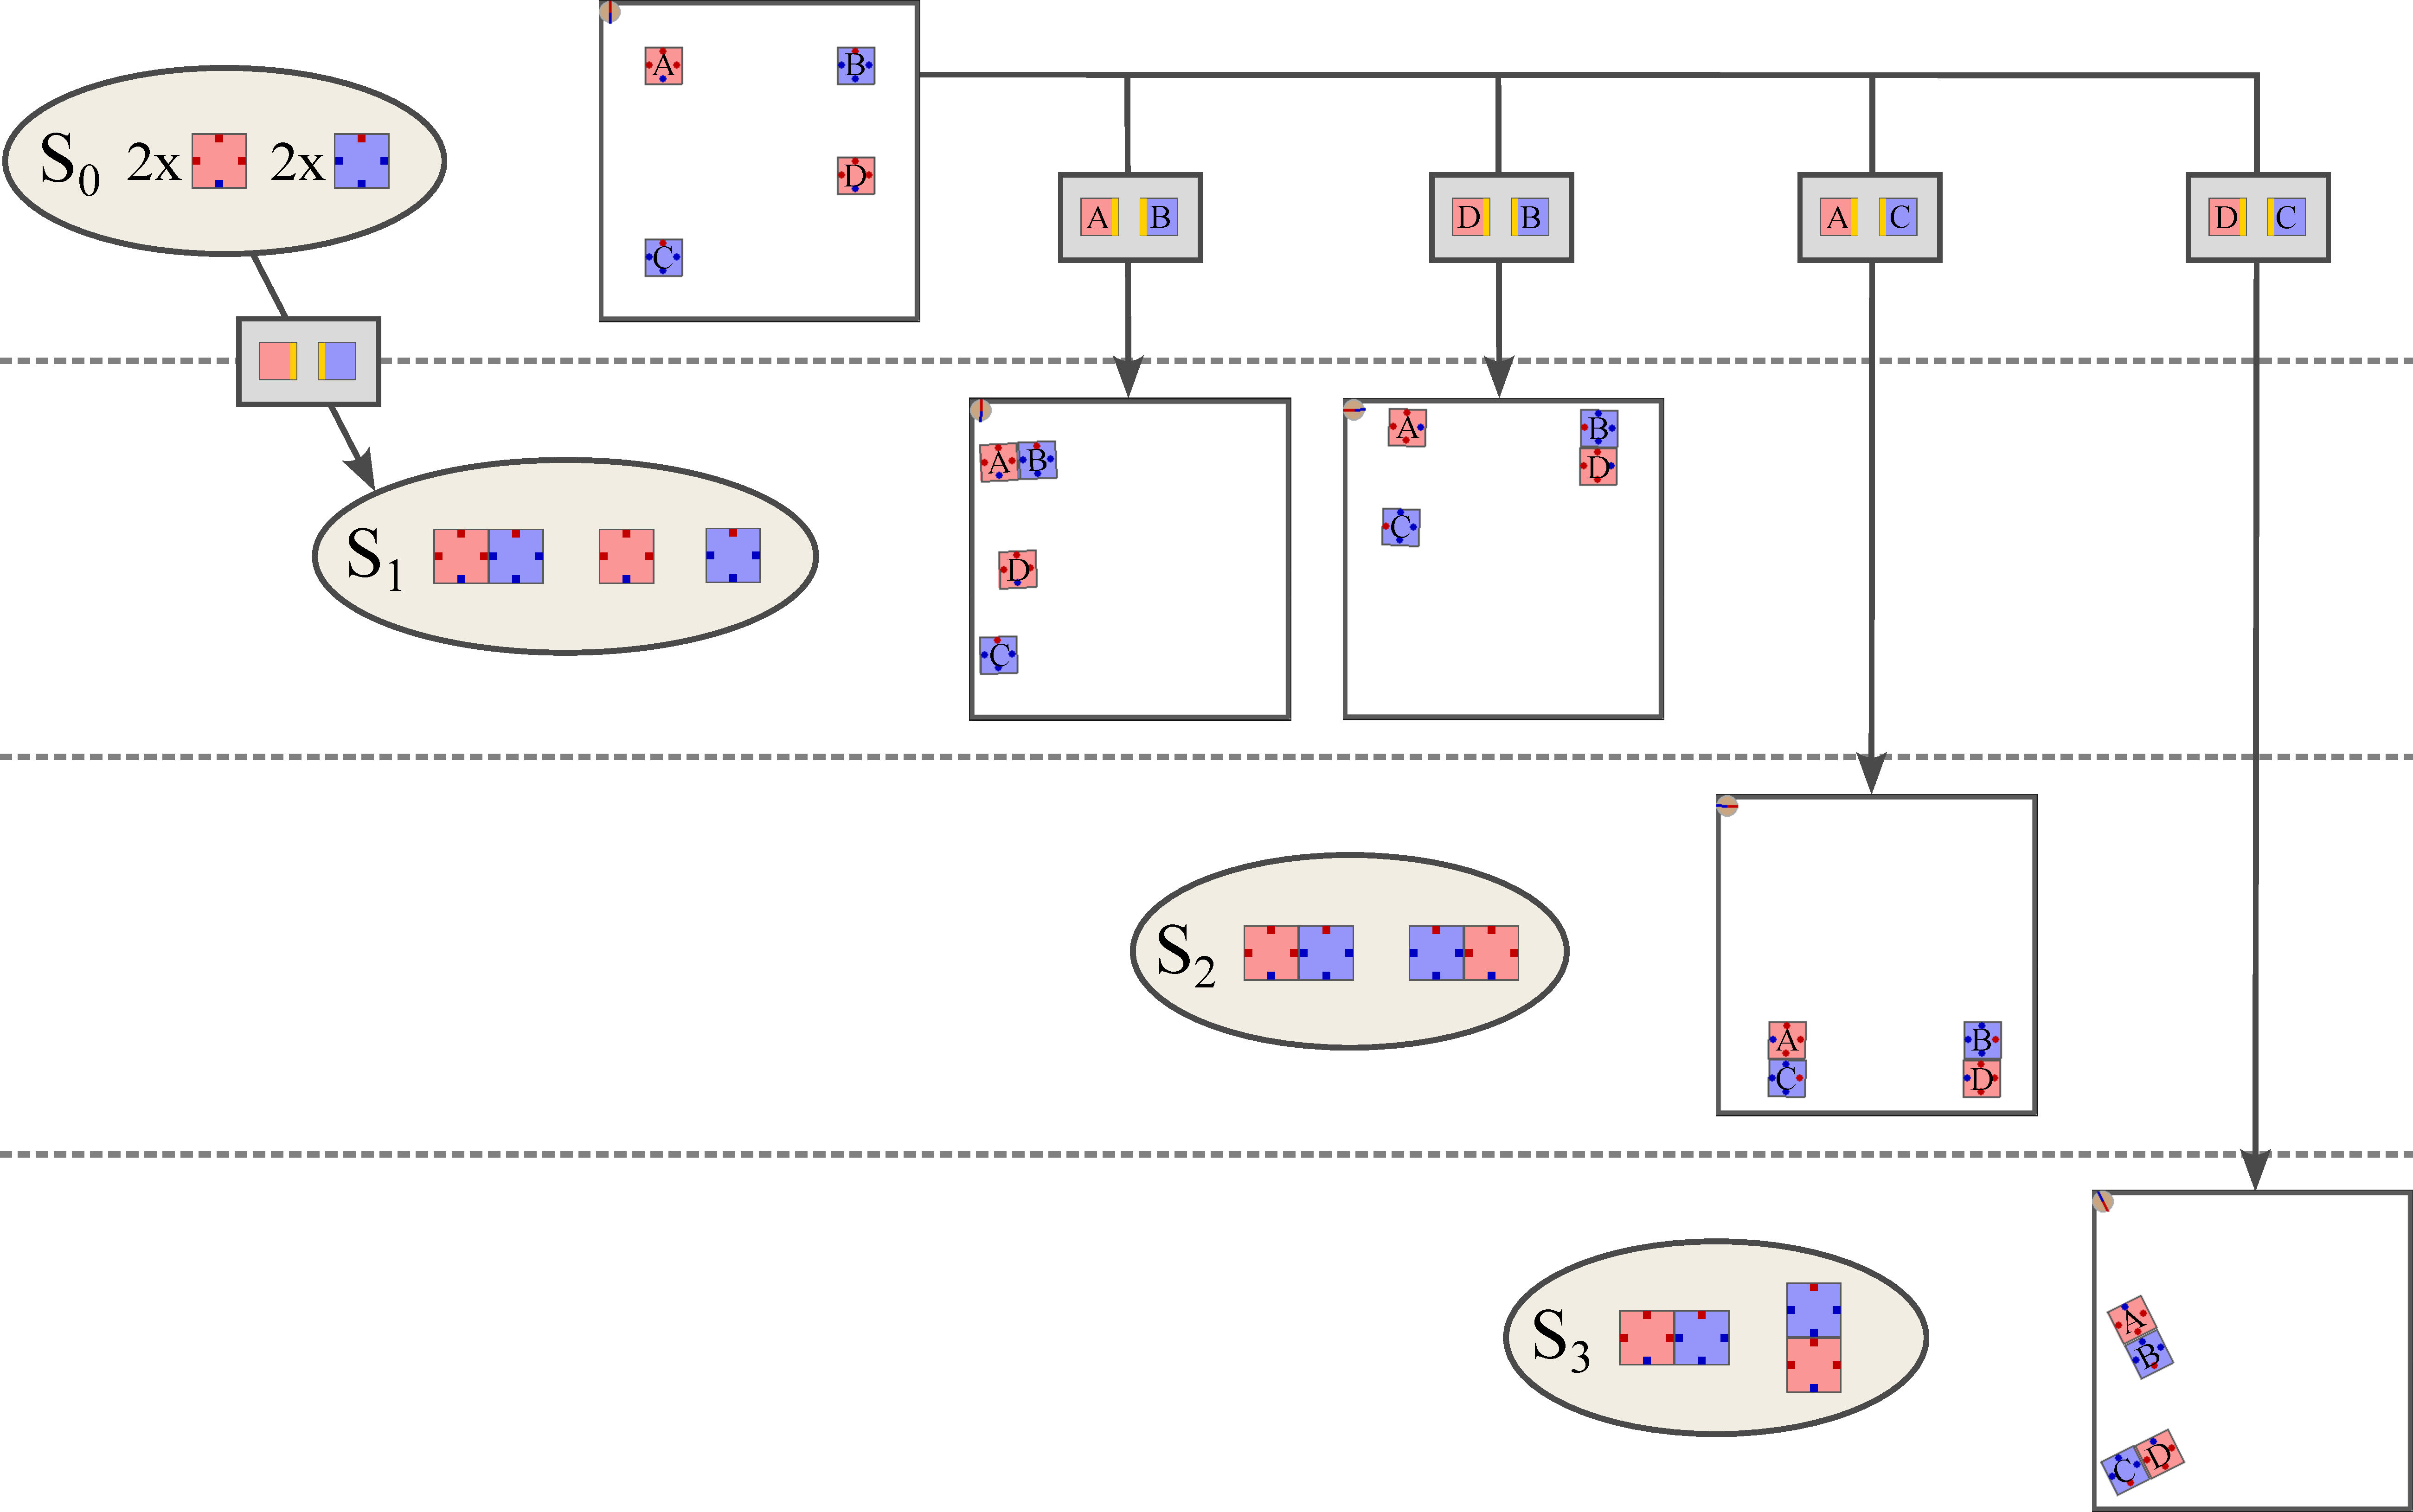
\includegraphics[width=1\textwidth]{figures/connect_options.pdf}
	\caption[Example of connection options for one two-cut-sub-assembly edge]{All connection options when connecting a red cube at the west of a blue cube to get from $S_7$ to $S_4$. Developing a local plan for different polyomino pairs, leads to different goal configurations. $(A_1,B_1)$ and $(A_2,B_1)$ lead to the desired polyomino set $S_4$, but $(A_2,B_2)$ leads directly to $S_2$. All these sets can be found in the TCSA graph of \autoref{fig:tcsa}. The goal configuration of $(A_1, B_2)$ holds the set $S_x$, which cannot be found in \autoref{fig:tcsa}. For further global planning this set could not be used.}
	\label{fig:connect_options}
\end{figure}

In each configuration $g$ the global planner encounters, $G_{\textit{TCSA}}(\mathcal{T})$ will be used to determine the next connection, that the local planner should try to establish.
$G_{\textit{TCSA}}(\mathcal{T})$ will be searched for the node that is the polyomino set $S(g)$.
If $S(g) \notin G_{\textit{TCSA}}(\mathcal{T})$, $g$ cannot be used to assemble $\mathcal{T}$.
This also allows the global planner to state failure immediately, when a initial configuration already contains sub-assemblies that are not usable for assembling $\mathcal{T}$.
With the exception of $S_\mathcal{T}$ all nodes have outgoing edges in a TCSA graph.
All outgoing edges of $S(g)$ provide connections for the local planner that bring the global planner closer to assembling $\mathcal{T}$.

For instance, if $S(g) = S_7$ in \autoref{fig:tcsa}, three outgoing edges provide three connections to choose from, but that is not all.
Assume the global planner decides to connect a red cube at the west edge of a blue cube to end up in a configuration $g_2$ with $S(g_2) = S_4$.
Since $S_7$ contains multiple polyominoes for the same type, there is more than one way to achieve this.
\autoref{fig:connect_options} illustrates all the different connection options for this example case.
You can also see how theses options differ in the goal configurations the local planner ended in.

Let $L_\mathcal{A}$ and $L_\mathcal{B}$ be collections of the physically distinct polyominoes for the polyomino types $\mathcal{A}$ and $\mathcal{B}$.
When $\mathcal{A}$ and $\mathcal{B}$ are about to be connected as the weight of a TCSA edge dictates, there are $\left| L_\mathcal{A} \times L_\mathcal{B} \right|$ polyomino pairs to choose from.
If $\mathcal{A} = \mathcal{B}$, the options where a polyomino will be connected with itself can be eliminated.

With multiple edges and various polyomino pairs per edge, many options emerge for the global planner to consider.
We examined three option sorting strategies for these options, to provide an order of the best probable outcome that the global planner can work through. 
We define functions for determining the best option $\hat{o}$ out of two options $o_1$ and $o_2$.
The approaches are compared in \autoref{chap:results}.

\paragraph{Minimal Distance}

The minimal distance sorting sorts connection options based on the distance between the cubes that are about to be connected.
The idea is that a smaller distances requires less movement to connect, which means shorter simulation time and lower plan costs of the resulting plan.
Due to sliding on walls and different pivot walking distances, this is not true in every case, but it remains a good heuristic for sorting.
Less movement might even prevent unwanted sub-assemblies.
\begin{equation}
\hat{o}(o_1, o_2) =
\begin{cases}
o_1 & \text{if } d(c_{\mathcal{A},1}, c_{\mathcal{B},1}) \leq d(c_{\mathcal{A},2}, c_{\mathcal{B},2}) \\
o_2 & \text{otherwise}
\end{cases}
\end{equation}

\paragraph{Grow Largest Component}

Another approach is to grow the largest component.
The options are sorted into classes of maximum polyomino size $\hat{n}$ of the resulting polyomino set.
We prefer TCSA edges that lead to sets containing the biggest polyominoes.
When the options for $S_4$ in \autoref{fig:tcsa} are sorted, the one leading to $S_1$ is preferred over the one leading to $S_2$, because $S_1$ contains a polyomino of size $3$, while $S_2$ only contains polyominoes of size $2$. 
The options within each class are sorted with the minimal distance approach.

If no other sub-assemblies occur, growing the largest component behaves like one-tile-at-a-time assembly.
The benefit is, that even if they occur the TSCA graph can provide solutions to integrate them if possible.
Larger polyominoes generally move faster acting positive on plan costs.

\begin{equation}
\hat{o}(o_1, o_2) =
\begin{cases}
o_1 & \text{if } \hat{n}_1 > \hat{n}_2 \lor \left( \hat{n}_1 = \hat{n}_2 \land d(c_{\mathcal{A},1}, c_{\mathcal{B},1}) \leq d(c_{\mathcal{A},2}, c_{\mathcal{B},2})\right) \\
o_2 & \text{otherwise}
\end{cases}
\end{equation}

\paragraph{Grow Smallest Component}

Oppositely to growing the largest component, options can be sorted by the smallest maximum size of polyominoes in polyomino sets.
This avoids working with large polyominoes, which are faster, but also need more simulation time to perform rotations and can be hard to handle, because of sheer size.

\begin{equation}
\hat{o}(o_1, o_2) =
\begin{cases}
o_1 & \text{if } \hat{n}_1 < \hat{n}_2 \lor \left( \hat{n}_1 = \hat{n}_2 \land d(c_{\mathcal{A},1}, c_{\mathcal{B},1}) \leq d(c_{\mathcal{A},2}, c_{\mathcal{B},2})\right) \\
o_2 & \text{otherwise}
\end{cases}
\end{equation}

\section{Use of Local Planner}
\label{sec:local_in_global}

The local planner develops plans for connections chosen from the different connection options presented in \autoref{sec:connect_options}.
For the local planner only one connection, out of the path of connections stored in the weight of a TSCA edge, needs to be picked.
Whenever a path consists of both north-south and east-west connections, a north-south connection is preferred.
This is done to perform offset-aligning instead of straight-aligning (\autoref{sec:align}), for an easier slide-in.
Besides of that, the choice of connection is irrelevant, since all connections in the path lead to the same outcome.

When the local planner successfully connects the desired polyominoes, other sub-assemblies can lead to a different polyomino set than expected.
This is not necessarily bad, as long as the resulting set is contained in $G_{\textit{TCSA}}(\mathcal{T})$.
In-fact, more sub-assemblies decrease the number of polyominoes in the workspace, which brings the goal of assembling $\mathcal{T}$ even closer.
Layers of depth were skipped in the TCSA graph, so that it might be possible to assemble $\mathcal{T}$ with less than $n-1$ local plans.
This can be seen in \autoref{fig:connect_options}, where $A_2$ and $B_2$ were connected. 
The resulting polyomino set matches with $S_2$ instead of $S_4$ of the nodes from \autoref{fig:tcsa}.

Like already mentioned in \autoref{sec:connect_options}, when the resulting polyomino set is not in $G_{\textit{TCSA}}(\mathcal{T})$, it is not possible to assemble the target from that configuration.
This can be seen in \autoref{fig:connect_options} when connecting $A_1$ and $B_2$.
For global use we add a new failure condition to the local planner, which checks if the polyomino set of the configuration in the workspace is contained in $G_{\textit{TCSA}}(\mathcal{T})$.
If not, the planner immediately states failure and avoids spending simulation time on a configuration with no further use.

The local planner might even fail to establish the desired connection.
If the resulting polyomino set is contained in $G_{\textit{TCSA}}(\mathcal{T})$, global planning can continue, but there are certain failure types that are not valid for further planning.
Polyomino sets with invalid polyominoes, or where connections in caves are necessary, should not be present in the TCSA graph anyway, but we also do not continue planning with a failure due to maximum movement capacity or polyominoes being stuck.

\section{Global Planning Algorithm}
\label{sec:global_algo}

\begin{algorithm}
	\caption{\scshape Assemble-Target}
	\label{algo:global_algo}
	\begin{algorithmic}[1]
		\REQUIRE $\mathcal{T}$, $g_\textit{init}$ \COMMENT{target polyomino and intital configuration}
		\ENSURE $s$, $P$ \COMMENT{state of global plan $s$ and plan stack $P$ containing local plans}
		\STATE $G_{\textit{TCSA}}(\mathcal{T}) \gets \text{\scshape Build-TCSA-Graph}(\mathcal{T})$
		\STATE $s \gets \text{undefined}$
		\STATE $P \gets \{\}$ 
		\STATE $g \gets g_\textit{init}$ \COMMENT{current configuration $g$}
		\LOOP
			\STATE $O \gets \text{\scshape Connection-Options}(g, G_{\textit{TCSA}}(\mathcal{T}))$
			\STATE valid $\gets$ \FALSE
			\WHILE[try options until local plan is valid]{\NOT $\text{\scshape Empty}(O)$ \AND \NOT valid}
				\STATE $(c_\mathcal{A}, c_\mathcal{B}, e_\mathcal{A}, e_\mathcal{B}) \gets \text{\scshape Pop}(O)$
				\STATE $p_\textit{new} \gets \text{\scshape Local-Planner}(g, (c_\mathcal{A}, c_\mathcal{B}, e_\mathcal{A}, e_\mathcal{B}), G_{\textit{TCSA}}(\mathcal{T}))$
				\IF{$\text{\scshape Valid-Plan}(p_\textit{new})$}
					\STATE valid $\gets$ \TRUE
				\ENDIF
			\ENDWHILE
			\IF{valid}
				\STATE $P \gets \text{\scshape Push}(P, p_\textit{new})$ \COMMENT{add new plan to plan stack}
				\STATE $g \gets g_\textit{goal}$ of new local plan $p_\textit{new}$ \COMMENT{move to new goal configuration}
				\IF[target got assembled]{$\mathcal{T} \in S(g)$}
					\STATE $s \gets \text{success}$
					\RETURN $(s, P)$
				\ENDIF
			\ELSE
				\IF[no configuration to fall back to]{$\text{\scshape Empty}(P)$}
					\STATE $s \gets \text{failure}$
					\RETURN $(s, P)$
				\ENDIF
				\STATE $p_\textit{pre} \gets \text{\scshape Pop}(P)$ \COMMENT{remove last plan from plan stack}
				\STATE $g \gets g_\textit{init}$ of last local plan $p_\textit{pre}$ \COMMENT{fall back to last initial configuration}
			\ENDIF
		\ENDLOOP
	\end{algorithmic}
\end{algorithm}

The global planning algorithm provided in \autoref{algo:global_algo} takes the initial configuration $g_\textit{init}$ and the target $\mathcal{T}$ as inputs and returns the state of the global plan $s$ and a plan stack $P$ as outputs.
For a successful plan, $P$ contains the local plans leading to the assembly of $\mathcal{T}$.
When concatenating the actions of all the plans in $P$, this creates a sequence of actions, that together form the global plan.
Because the local plans were created by using a TCSA graph, $|P| < n$ holds true (\autoref{sec:local_in_global}).
The reason for $P$ being called a stack is the way it is used in \autoref{algo:global_algo}.
The algorithm explores the configuration-space along $G_{\textit{TCSA}}(\mathcal{T})$ in a depth-first-search manner, which is done in the attempt to get closer to assembling $\mathcal{T}$ each iteration.

The algorithm starts with $g_\textit{init}$ as the current configuration $g$.
At first all the connection options for $g$ are determined with {\scshape Connection-Options} the way it was described in \autoref{sec:connect_options}.
The mechanisem behind this function can be viewed as a hash-map, storing the options as the values for the configuration as the key.
The options need to be determined and sorted, only when it is the first time a configuration is encountered.
The list of connection options $O$ that {\scshape Connection-Options} provides, is only a view on the values stored in the hash-map, meaning that when $O$ is altered, the hash-map is updated as well.
Whenever a connection option is popped from $O$, this option is removed from the hash-map and will therefore never be considered again.
Note that options are stored per configuration $g$, not for the polyomino set $S(g)$.
Two configuration sharing the same polyomino set both have their own lists of connection options.
We traverse the configuration-space with the TCSA graph as a guidance, not the TCSA graph itself.
Nodes in $G_{\textit{TCSA}}(\mathcal{T})$ can be encountered multiple times and will never be eliminated from planning.

Once the list of connection options $O$ is retrieved, the algorithm works through it in the order determined by the option sorting that was applied in advance.
This is done until a valid local plan was found, or no options are left.
{\scshape Local-Planner} uses \autoref{algo:local_algo} to create a local plan $p_\textit{new}$.
It also takes $G_{\textit{TCSA}}(\mathcal{T})$ as an input parameter, to ensure the newly added failure condition, when a configurations polyomino set is not contained in $G_{\textit{TCSA}}(\mathcal{T})$.
The validity of a local plan is evaluated with {\scshape Valid-Plan}.

If a valid local plan was found, $p_\textit{new}$ is pushed on to $P$ and $g$ is set to the goal configuration of $p_\textit{new}$.
When a configuration containing $\mathcal{T}$ is reached, the global plan is successful and the algorithm returns.
On the other hand, if no valid option for $g$ could be found, the algorithm has to fall back to the last visited configuration.
For that the top local plan $p_\textit{pre}$ on $P$ is popped and its initial configuration becomes the new $g$.
Even though $p_\textit{pre}$ was a successful local plan, it led to a dead end and had to be removed from the stack.
If $P$ is empty the current configuration is $g_\textit{init}$.
This means that there is no previously visited configuration the algorithm can fall back to.
In that case the algorithm has to state failure for assembling $\mathcal{T}$.

Before calling \autoref{algo:global_algo} checking if $\mathcal{T} \in S(g_\textit{init})$ is necessary, to state early success.
Furthermore, a timeout failure is added to \autoref{algo:global_algo}, in case planning takes to long.
 
\subsection{Complexity}
\label{sec:global_complex}

\paragraph{Optimality}

Given that the local planner does not produce an optimal solution for the connection of two polyominoes, the global planner will also not reach optimality.
Even if the local planner provides only optimal solutions, our depth-first-search approach would not explore the configuration space in a way that the best sequence of local plans is guaranteed to be picked.
\autoref{algo:global_algo} greedily moves along the depth of the TCSA graph to assemble the target as fast as possible.
The option sorting strategies provide reasonable heuristics for picking a connection option per individual TCSA node, but cannot ensure the optimal decision, let alone the optimal decision for the whole path of connection options taken.
Optimal solutions would need broad exploration and comparison of different paths to the target, which is infeasible in our case due to the high simulation time required for local plans.

\paragraph{Completeness}

The same as with optimality, the local planner prevents the completeness of the global planner.
Assuming completeness of the local planner, the global planner could be certain of the existence or non-existence of a solution for assembling $\mathcal{T}$.
\autoref{algo:global_algo} will always return success or failure in finite time.
This is due to the finite number of connection options per configuration and the depth $n$ of the TCSA graph.
Each local plan in the plan stack is certain to connect at least two polyominoes, so after $n-1$ local plans the workspace contains only one $n$-size polyomino.
This polyomino is not necessarily $\mathcal{T}$, but no further connections can be made, which makes the algorithm fall back to the last configuration.
Together with the finite number of options per configuration, the algorithm will eventually explore all paths of connection options that are possible and can therefore verify the existence or non existence of a solution.
Remember that this completeness is based purely on the strong assumption of a complete local planer, which is challenging to archive in the special Euclidean group.

\paragraph{Efficiency}

We have to differentiate between local plans in the plan stack and local plans created during planning $\#\textit{local}$.
Even though $|P| < n$, the global planner might have created more local plans, which were either invalid or had to be removed, because they lead to a dead end.
In a best case only one local plan could lead to the assembly of $\mathcal{T}$.
This is highly unrealistic, but theoretically possible, since layers of depth in the TCSA graph can be skipped.
A more realistic best case would be $n-1$ local plans created during planning. 
This would assume, that all local plans created were valid and lead directly to the target with no layer skipping.

In a worst case all paths of connection options have to be explored before stating failure.
In this worst case ``all'' means that each connection option at each configuration produces a valid local plan with no other sub-assemblies leading to a unique new configuration.
The only invalid local plans are the ones that lead to a configuration with one $n$-size polyomino that is not $\mathcal{T}$.
It is not possible to state the exact amount of worst case local plans, since the number of connection options per configuration varies.
By taking the average number of connection options per TCSA node $o_\mu$, we can define an estimate

\begin{equation}
\#\textit{local}_\textit{worst} = \sum_{i=1}^{n-1} {o_\mu}^i \, .
\end{equation} 
For $n = 10$ and $o_\mu = 20$ this results in $\#\textit{local}_\textit{worst} \approx 5 \cdot 10^{11}$.

It is impossible to simulate that many local plans in a reasonable time.
For that reason a timeout failure was added.
\autoref{chap:results} will provide experimental data on the number of $\#\textit{local}$ and what percentage of global plans time out.
The number of configurations explored $\#\textit{config}$ is also examined in the experiments to better portray the number of dead ends during planning.


\section{More Cubes than Target}
\label{sec:more_cubes}

The number of cubes in the workspace is limited to the target size $n$ for the global planner to work.
The reason for this is linked with the use of TCSA graphs. 
Using a hash-table to find a TCSA node $S_\textit{TCSA}$ and check for equality with the configurations polyomino set $S(g)$ is simple and fast.
If a configuration holds more cubes then the TCSA nodes hold, we need to check if $S_\textit{TCSA} \subseteq S(g)$.
This cannot be done by hash comparing, so all nodes of the graph need to be checked, which would be very costly.
In addition to that, multiple nodes can be included in $S(g)$.
The global planner could handle this by summing up the connection options of all the nodes, but again this makes planning more complex and costly.

After assembling $\mathcal{T}$ all the leftover cubes could assemble various polyominoes.
We could enumerate all possible left over polyomino sets $S_l$ and remove all of them separately from $S(g)$ to check for $S_\textit{TCSA} = S(g) \setminus S_l$.
This would again result in multiple nodes and summed up connection options, but with the ability to hash compare for equality.
The number of $S_l$ can become huge for increasing numbers of leftover cubes leading to a less efficient global planner.




